\documentclass[fontsize=6pt,DIV=calc,a4paper,ngerman]{scrartcl}


\usepackage{avant}
\renewcommand*\familydefault{\sfdefault} %% base font



\usepackage[T1]{fontenc}
\usepackage{multicol,blindtext,amsmath,amsfonts,amssymb,bm,leftidx}
\usepackage[a4paper,landscape]{geometry}
\usepackage{graphicx,tabularx,trfsigns,makecell}
\usepackage[dvipsnames]{xcolor}

\usepackage[ruled,vlined]{algorithm2e}
%Example Algorithm
%\begin{algorithm}[H]
%    \SetAlgoLined % set vertical lines from while to end
%     $ formula $ \tcp*{Side Comment}
%     \While{$a > b$}{ 
%     $ formula $ \tcp*{Side Comment}
%     }
%     \caption{Algorithm Title}
%\end{algorithm}



\geometry{hmargin=0.7cm, top=0.7cm, bottom=0.4cm,includefoot} %small borders
\setlength\columnseprule{0.5pt} %line between columns

\newcommand{\mathbbm}[1]{\text{\usefont{U}{bbm}{m}{n}#1}} %Font for unit Matrix

\parindent 0pt %Texteinzug erste Zeile



%TITLE Formating
\usepackage{titlesec}
\titleformat{\section}
  {\normalfont\Large\bfseries\color{PineGreen}}{\makebox[25pt][l]{\thesection}}{0pt}{}[{\titlerule[1pt]}]
\titleformat{\subsection}
  {\normalfont\large\bfseries\color{OliveGreen}}{\makebox[25pt][l]{\thesubsection}}{0pt}{}
\titleformat{\subsubsection}
  {\normalfont\normalsize\bfseries\color{TealBlue}}{\makebox[25pt][l]{\thesubsubsection}}{0pt}{}


\setcounter{section}{-1} %start with section 0

\begin{document}

\begin{multicols*}{4}
	% \title{Summary Robot Dynamics}
	% \author {Adrian Hartmann}
	% \date {HS 2020 - Prof. Hutter}
	% \maketitle

	%%%%%%%%%%%%%%%%%%%%%%%%%%%%%%%%%%%%%%%%%%%%%%%%%%%%%%%%%%%%%%%%%%%%%%%%%%%%%%%%%%%%%%%%%%%%%%%%%%%%%%%%%%%%%%%%%%%
	%  _____           _   _               __ 
	% / ____|         | | (_)             /_ |
	%| (___   ___  ___| |_ _  ___  _ __    | |
	% \___ \ / _ \/ __| __| |/ _ \| '_ \   | |
	% ____) |  __/ (__| |_| | (_) | | | |  | |
	%|_____/ \___|\___|\__|_|\___/|_| |_|  |_|
	%%%%%%%%%%%%%%%%%%%%%%%%%%%%%%%%%%%%%%%%%%%%%%%%%%%%%%%%%%%%%%%%%%%%%%%%%%%%%%%%%%%%%%%%%%%%%%%%%%%%%%%%%%%%%%%%%%%

	\section{Basics}
	\begin{itemize}
		\item[] Vector from point B to P in frame $\mathcal{A}$: \quad $ {}_\mathcal{A} r_{BP}$
		\item[] Reference coordinate System $\mathcal{A}$: \quad $(e^{\mathcal{A}}_x,e^{\mathcal{A}}_y,e^{\mathcal{A}}_z)$
	\end{itemize}
	\textbf{Cartesian Coordinates}
	$$\text{Stacked parameters of Position:  }\chi_{Pc}=\begin{pmatrix}x\\y\\z\end{pmatrix}$$
	$$\text{Postion Vector: } {}_\mathcal{A}r = xe^{\mathcal{A}}_x+ye^{\mathcal{A}}_y+ze^{\mathcal{A}}_z = \begin{pmatrix}x\\y\\z\end{pmatrix}$$

	\begin{minipage}{0.45\linewidth}
		\textbf{Cylindric Coordinates}
		$$\scriptstyle\chi_{Pz}=\begin{pmatrix}\rho\\\theta\\z\end{pmatrix} ;\quad {}_\mathcal{A}r = \begin{pmatrix}\rho \, cos\theta\\\rho\, sin\theta \\ z\end{pmatrix}$$
	\end{minipage}
	\begin{minipage}{0.5\linewidth}
		\textbf{Spherical Coordinates}
		$$\scriptstyle \chi_{Ps}= \begin{pmatrix} r\\\theta \\ \phi\end{pmatrix}; \quad {}_\mathcal{A}r = \begin{pmatrix}r\, cos\theta\, sin\phi\\r\, sin\theta\, sin\phi \\ r\, cos\phi\end{pmatrix}$$
	\end{minipage}

	\section{Kinematics}
	\subsection{Linear Velocity}
	The Velocity of point B relative to point A is given by: $\quad \dot{r}_{AB}$.
	There exists a linear mapping $E_p(\chi)$ between velocities $\dot{r}$ and the derivatives of the representation $\dot{\chi}_P$:
	\begin{align*}
		\dot{r}      & = E_P(\chi_P)\dot{\chi}_P \\
		\dot{\chi}_P & = E^{-1}_P(\chi_P)\dot{r}
	\end{align*}
	For \textbf{Cartesian} this is the identity: $E_{Pc}(\chi_{Pc})=E_{Pc}^{-1}(\chi_{Pc})=\mathbbm{1}$

	In \textbf{Cylindrical} we get:

	$E_{Pz} = \frac{\partial r(\chi)}{\partial\chi} =
		\left(\begin{smallmatrix}c\theta &  -\rho\,s\theta & 0 \\ s\theta & \rho\,c\theta & 0\\ 0 & 0& 1\end{smallmatrix}\right)
		;\quad E_{Pz}^{-1} = \left(\begin{smallmatrix}c\theta & s\theta & 0 \\ -\frac{1}{\rho}s\theta& \frac{1}{\rho}c\theta & 0 \\ 0 & 0 & 1\end{smallmatrix}\right)$

	For \textbf{Spherical}:\\
	\begin{minipage}{0.5\linewidth}
		$E_{Ps} = $\\
		$\left(\begin{smallmatrix}
					c\theta\,s\phi & -r\,s\theta\,s\phi & r\, c\theta\,c\phi \\
					s\theta\,s\phi & r\,c\theta\,s\phi & r\, s\theta\,c\phi \\
					c\phi & 0 & -r\,s\phi
				\end{smallmatrix}\right)$
	\end{minipage}
	\begin{minipage}{0.5\linewidth}
		$E_{Ps}^{-1} =$\\
		$ \left(\begin{smallmatrix}
					c\theta\,s\phi & s\theta s\phi & c\phi \\
					-s\theta /(r\,s\phi) & c\theta/(r\,s\phi) & 0 \\
					\frac{1}{r} c\theta\,c\phi & \frac{1}{r}s\theta\,c\phi & -\frac{1}{r}s\phi
				\end{smallmatrix}\right)$
	\end{minipage}


	\subsection{Rotation}
	Orientation of frame $\mathcal{B}$ with reference to frame $\mathcal{A}$: $$\phi_{\mathcal{AB}}\in SO(3)$$
	\textcolor{red}{\textbf{Important:} There is no numerical equivalent to a position such as "angular position". Instead the orientation can be parametrized in several ways.}


	\begin{description}
		\item[Passive Rotation:] Passive rotations are transformations between different coordinate frames. ${}_\mathcal{A}u=C_\mathcal{AB}\cdot {}_\mathcal{B}u$
		\item[Active Rotations:] Active rotations contain an operator (i.e. $R\in \mathbbm{R}^{3\times 3})$ to rotate a vector in the same frame. ${}_\mathcal{A}v = R\cdot {}_\mathcal{A}u$
	\end{description}

	\subsubsection{Rotation Matrix}
	Mapping Coordinates P from frame $\mathcal{B}$ to $\mathcal{A}$:
	\begin{align*}
		{}_\mathcal{A}r_{AP} & = \begin{pmatrix}{}_\mathcal{A}e^{\mathcal{B}}_x & {}_\mathcal{A}e^{\mathcal{B}}_y & {}_\mathcal{A}e^{\mathcal{B}}_z\end{pmatrix}\cdot {}_\mathcal{B}r_{AP}
		\\
		                     & = C_{\mathcal{AB}}\cdot {}_\mathcal{B}r_{AP}
	\end{align*}
	This matrix is orthogonal: $C_\mathcal{BA} = C_\mathcal{AB}^{-1}=C_\mathcal{AB}^T$

	\subsubsection{Elementary Rotations}
	\begin{center}
		Around X-Axis \qquad Around Y-Axis \qquad Around Z-Axis
	\end{center}
	$$
		\setlength\arraycolsep{2pt} %lower space between columns
		\begin{pmatrix}
			1 & 0       & 0        \\
			0 & cos\phi & -sin\phi \\
			0 & sin\phi & cos\phi
		\end{pmatrix}
		\begin{pmatrix}
			cos\phi  & 0 & sin\phi \\
			0        & 1 & 0       \\
			-sin\phi & 0 & cos\phi
		\end{pmatrix}
		\begin{pmatrix}
			cos\phi & -sin\phi & 0 \\
			sin\phi & cos\phi  & 0 \\
			0       & 0        & 1
		\end{pmatrix}
	$$


	\subsubsection{Homogeneous Transformation}
	Combined Translation and Rotation for frames with a offset. The vector ${}_\mathcal{A}r_{AB}$ points from the origin of frame $\mathcal{A}$ to the origin of the $\mathcal{B}$ in frame $\mathcal{A}$. $T_\mathcal{AB}$ transforms a \textbf{point P} from frame $\mathcal{B}$ to $\mathcal{A}$.
	$$\begin{pmatrix}{}_\mathcal{A}r_{AP} \\ 1\end{pmatrix}= \underbrace{
			\begin{bmatrix}C_\mathcal{AB} & {}_\mathcal{A}r_{AB} \\
				0_{1\times3}   & 1
			\end{bmatrix}}_{T_\mathcal{AB}} \begin{pmatrix}
			{}_\mathcal{B}r_{BP} \\
			1
		\end{pmatrix}$$

	$$\text{With inverse: } T^{-1}_\mathcal{AB} = \left[\begin{smallmatrix}
				C_\mathcal{AB}^T & \overbrace{-C_\mathcal{AB}^T\,{}_\mathcal{A}r_{AB}}^{{}_\mathcal{B}r_{BA}} \\
				0_{1\times3} & 1
			\end{smallmatrix}\right]$$

	\subsection{Representation of Rotations}
	\subsubsection{Euler Angles}

	Rotation Matrix from Euler Angles:
	$$ C_{AD} = C_{AB}(z) C_{BC}(y) C_{CD}(x) $$

	Euler Angles from Rotation Matrix:
	$$\chi_{\text{R, eulerZYX}}
		= \begin{pmatrix} z \\ y \\ x \end{pmatrix}
		= \begin{pmatrix}
			\text{atan2}(c_{21}, c_{11})                      \\
			\text{atan2}(-c_{31}, \sqrt{x_{32}^2 + c_{33}^2}) \\
			\text{atan2}(c_{32}, c_{33})
		\end{pmatrix}
	$$

	% Euler Angles describe a rotation as a sequence of 3 elementary rotations. When the first and the last rotations are made around the same axis, the parametrisation is called \textbf{proper Euler angles}. For three different Axis we typically refer to \textit{Tait-Bryan}, \textit{Cardan} or \textit{roll-pitch-yaw} angles.

	\subsubsection{Angle Axis}
	$$\chi_{R,\text{AngleAxis}}=\begin{pmatrix}\theta \\ \overrightarrow{n}\end{pmatrix} \; \textbf{Rotation Vector: } \varphi = \theta\cdot\overrightarrow{n}$$

	Rotation Matrix from Angle Axis:
	$$ C_{AB} = \cos(\theta) I_{3\times3} - \sin(\theta) [n]_\times  + (1- \cos(\theta)) nn^T $$

	Parameters from Rotation Matrix:
	$$ \theta = \cos^{-1} \left( \frac{c_{11} + c_{22} + c_{33} - 1}{2} \right);
		n = \frac{1}{2\sin(\theta)}
		\begin{pmatrix}
			c_{32} - c_{23} \\
			c_{13} - c_{31} \\
			c_{21} - c_{12}
		\end{pmatrix} $$

	\subsubsection{Unit Quaternion}
	A non-minimal representation which doesn't suffer from sigularites

	From rotation vector $\varphi \in \mathbb{R}^3$ to unit quaternion:
	$$\chi_{R,quat}= \xi =\begin{pmatrix}\xi_0 \\ \check{\xi}\end{pmatrix} =
		\begin{pmatrix}
			cos(\frac{\theta}{2}) \\
			sin(\frac{\theta}{2}) \overrightarrow{n}
		\end{pmatrix} =
		\begin{pmatrix}\xi_0 \\ \xi_1 \\ \xi_2 \\ \xi_3 \end{pmatrix}$$

	Hamiltonian conventions:
	$$ \xi = \xi_0 + \xi_1i + \xi_2j + \xi_3k \quad
	i^2 = j^2 = k^2 = ijk = -1; $$
	$$
	ij = -ji = -ijk^2 = k \quad
	jk = -kj = i \quad
	ki = -ik = j $$

	The first parameter $\xi_0$ is called the real part of the quaternion, the latter $\check{\xi}$ the imaginary part. The \textbf{unit} quaternion fulfils the constraint:
	$$\xi_0^2 + \xi_1^2 + \xi_2^2 +\xi_3^2 = 1$$
	Given a rotation matrix, the corresponding quaternion is:
	$$\chi_{R,quat}=\xi_\mathcal{AD}=\frac{1}{2}\left(\begin{smallmatrix}
				\sqrt{c_{11}+c_{22}+c_{33}+1}\\
				sgn(c_{32}-c_{23})\sqrt{c_{11}-c_{22}-c_{33}+1}\\
				sgn(c_{13}-c_{31})\sqrt{c_{22}-c_{33}-c_{11}+1}\\
				sgn(c_{21}-c_{12})\sqrt{c_{33}-c_{11}-c_{22}+1}
			\end{smallmatrix}\right)$$
	\begin{flushright}
		with $sgn(x) = 1$ for $x\geq 0$ and $sgn(x) = -1$ for $x<0$
	\end{flushright}

	The Corresponding Rotation Matrix can be calculated with:
	\begin{align*}
		C_\mathcal{AD} & = \mathbbm{1}_{3\times 3}+2\xi_0\, [\check{\xi}]_\times+2[\check{\xi}]_\times^2
		\\
		               & = (2\xi_0^2-1)\,\mathbbm{1}_{3\times 3} +2\xi_0 [\check{\xi}]_\times+2\check{\xi}\check{\xi}^T \\
		               & = \left(\begin{smallmatrix}
				\xi_0^2+\xi_1^2-\xi_2^2-\xi_3^2 & 2\xi_1\xi_2-2\xi_0\xi_3 & 2\xi_0\xi_2+2\xi_1\xi_3 \\
				2\xi_0\xi_3+2\xi_1\xi_2 & \xi_0^2-\xi_1^2+\xi_2^2-\xi_3^2 & 2\xi_2\xi_3-2\xi_0\xi_1 \\
				2\xi_1\xi_3-2\xi_0\xi_2 & 2\xi_0\xi_1-2\xi_2\xi_3 & \xi_0^2-\xi_1^2-\xi_2^2+\xi_3^2
			\end{smallmatrix}\right)
	\end{align*}

	It holds that:
	$$\xi = \begin{pmatrix}\xi_0 \\ \check{\xi}\end{pmatrix} \xrightarrow[]{inverse} \xi^{-1} = \xi^T =\begin{pmatrix}\xi_0 \\ -\check{\xi}\end{pmatrix}$$

	Multiplication: $ \xi_\mathcal{AB}\otimes \xi_\mathcal{BC} = M_l(\xi_\mathcal{AB}) \xi_\mathcal{BC}$
	$$
		\underbrace{\left(\begin{smallmatrix}
					\xi_0 & -\xi_1 & -\xi_2 & -\xi_3 \\
					\xi_1 & \xi_0 & -\xi_3 & \xi_2 \\
					\xi_2 & \xi_3 & \xi_0 & -\xi_1 \\
					\xi_3 & -\xi_2 & \xi_1 & \xi_0 & \\
				\end{smallmatrix}\right)_\mathcal{AB} }_{M_l(\xi_\mathcal{AB})}
		;
		\underbrace{\left(\begin{smallmatrix}
					\xi_0 & -\xi_1 & -\xi_2 & -\xi_3 \\
					\xi_1 & \xi_0 & \xi_3 & -\xi_2 \\
					\xi_2 & -\xi_3 & \xi_0 & \xi_1 \\
					\xi_3 & \xi_2 & -\xi_1 & \xi_0 & \\
				\end{smallmatrix}\right)_\mathcal{BC} }_{M_r(\xi_\mathcal{BC})}
	$$
	There exists a similar Matrix $M_r$ for right multiplications.

	\smallskip
	Direct way of rotating a Vector: (with $p({}_\mathcal{B}r)= \left(\begin{smallmatrix} 0 \\ {}_\mathcal{B}r\end{smallmatrix}\right)$)
	$$p({}_\mathcal{A}r)
		=\xi_\mathcal{AB} \otimes p({}_\mathcal{B}r) \otimes \xi^T_\mathcal{AB}
		=M_l(\xi_\mathcal{AB})M_r(\xi_\mathcal{AB}^T)p({}_\mathcal{B}r)$$

	\subsection{Angular Velocity}
	Consider Frame $\mathcal{B}$ which is moving with respect to fixed Frame $\mathcal{A}$. The angular velocity of the rotation of $\mathcal{B}$ w.r.t $\mathcal{A}$ is ${}_\mathcal{A}\omega_\mathcal{AB}$.

	It can be shown that: $$ [{}_\mathcal{A}\omega_\mathcal{AB}]_\times=\dot{C}_\mathcal{AB}\cdot C_\mathcal{AB}^T$$
	with $ [{}_\mathcal{A}\omega_\mathcal{AB}]_\times =
		\left(\begin{smallmatrix}
				0 & -\omega_z & \omega_y \\
				\omega_z & 0 & -\omega_x \\
				-\omega_y & \omega_x & 0
			\end{smallmatrix}\right)
	$ and ${}_\mathcal{A}\omega_\mathcal{AB}=\begin{pmatrix}\omega_x \\ \omega_y\\\omega_z	\end{pmatrix}$

	Angular Velocities can be transformed as normal vectors:
	$${}_\mathcal{B}\omega_\mathcal{AB}= C_\mathcal{BA}\cdot {}_\mathcal{A}\omega_\mathcal{AB}$$
	the product matrix is transformed by:
	$$[{}_\mathcal{B}\omega_\mathcal{AB}]_\times = C_\mathcal{BA}\cdot [{}_\mathcal{A}\omega_\mathcal{AB}]_\times\cdot C_\mathcal{AB}$$

	Angular Velocities in the same Frame can be added:
	$${}_\mathcal{I}\omega_\mathcal{IE}= {}_\mathcal{I}\omega_{\mathcal{I}0}+ ... + {}_\mathcal{I}\omega_{n\mathcal{E}}$$

	\subsubsection{Time Derivative of Rotation Parameters}
	Similarly to the linear velocity we can define:
	$${}_\mathcal{A}\omega_\mathcal{AB}=E_R(\chi_R)\cdot \dot{\chi}_R$$
	{\small i.e. quaternions:} $E_R = 2H(\xi)=2\left[ \begin{smallmatrix}-\check{\xi}\quad & [\check{\xi}]_\times + \xi_0\mathbbm{1}_{3\times 3}\end{smallmatrix}\right]\in \mathbb{R}^{3\times 4}$

	\subsection{Velocity in Moving Bodies}
	\begin{center}
		\begin{tabularx}{0.8\linewidth}{l|l}
			$v_P$                                       & the absolute Velocity of point P          \\
			$a_P=\dot{v}_P$                             & (absolute) acceleration of P              \\
			$\Omega_\mathcal{B}= \omega_\mathcal{AB}$   & (absolute) angular velocity of body B     \\
			$\Psi_\mathcal{B}=\dot{\Omega}_\mathcal{B}$ & (absolute) angular acceleration of body B
		\end{tabularx}
	\end{center}

	We can write the Position P as:
	$${}_\mathcal{A}r_{AP}={}_\mathcal{A}r_{AB}+C_\mathcal{AB}\cdot {}_\mathcal{B}r_{BP}$$
	Which can be differentiated to:
	$${}_\mathcal{A}\dot{r}_{AP}={}_\mathcal{A}\dot{r}_{AB}+{}_\mathcal{A}\omega_\mathcal{AB}\times {}_\mathcal{A}r_{BP}$$

	This is the famous \textbf{Rigid Body Formulation} for velocities:
	$$v_P=v_B+\Omega \times r_{BP}$$
	For Accelerations:
	$a_P=a_B+\Psi\times r_{BP}+\Omega\times(\Omega\times r_{BP})$

	\smallskip
	In case a moving system $\mathcal{B}$ is used for representation, the \textbf{Euler Differentiation rule} must be applied (with a non moving system $\mathcal{A}$):
	\begin{align*}
		{}_\mathcal{B}v_P
		 & = C_\mathcal{BA} \cdot \frac{d}{dt}(C_\mathcal{AB}\cdot {}_\mathcal{B}r_{AP})             \\
		 & = {}_\mathcal{B}\dot{r}_{AP}+{}_\mathcal{B}\omega_\mathcal{AB}\times {}_\mathcal{B}r_{AP}
	\end{align*}

	\subsection{Kinematics of Systems of Bodies}
	\subsubsection{Generalized Coordinates and Joint Configurations}
	The configuration of a root such as a manipulator can be described by the \textbf{generalized coordinate vector}: $q=\begin{pmatrix}q_1 &\dots & q_n\end{pmatrix}^T$
	The choice of q isn't unique, but it has to completely describe the configuration of the system (q const. $\Rightarrow$ robot can't move).

	\begin{center}
		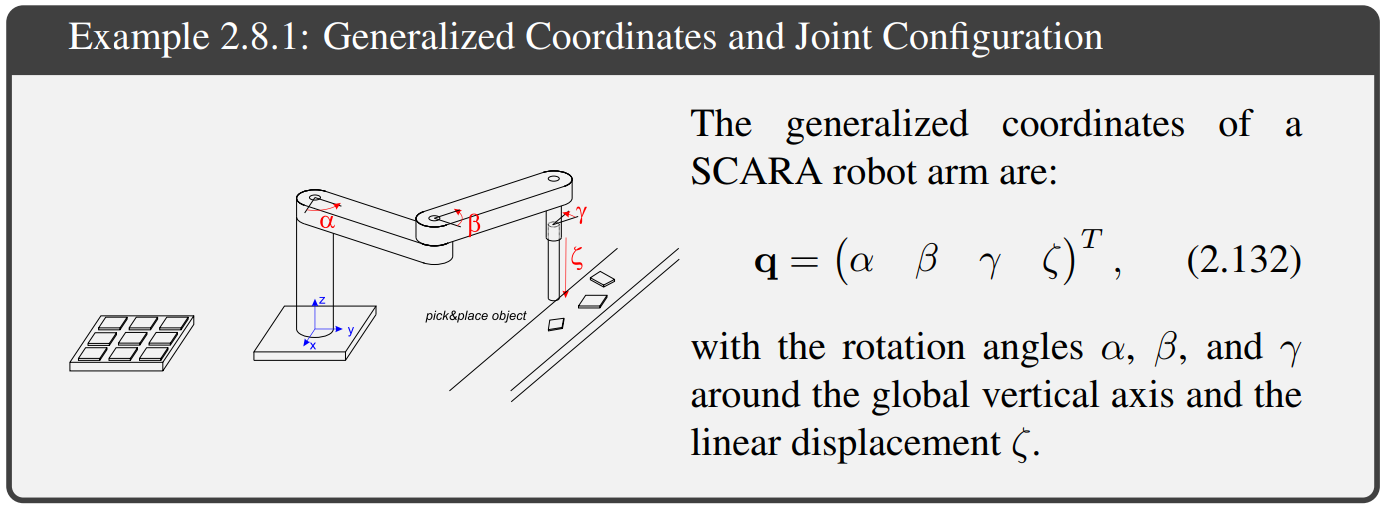
\includegraphics[width=0.8\linewidth]{general_coords_SCARA.png}
	\end{center}
	\subsubsection{Task-Space Coordinates}
	\textbf{End-Effector Configuration Parameters}

	The position $r_e\in \mathbb{R}^3$ and rotation $\phi_e \in SO(3)$ of a frame w.r.t a base can be parametrized by:
	$$\chi_e = \begin{pmatrix}\chi_{eP} \\ \chi_{eR}\end{pmatrix} = \left(\begin{smallmatrix}\chi_{1} \\\vdots \\\chi_{m}\end{smallmatrix}\right)\in \mathbb{R}^m$$

	\textbf{Operational Space Coordinates}
	The end-effector operates in the operational space, which depends on the geometry and structure of the arm. It can be described with:
	$$\chi_o = \begin{pmatrix}\chi_{oP} \\ \chi_{oR}\end{pmatrix}=\left(\begin{smallmatrix}\chi_{1} \\\vdots \\\chi_{m_o}\end{smallmatrix}\right)$$
	where $\chi_1 \dots \chi_{m_o}$  are \textit{independent} operational space coordinates. It can be seen as a \textbf{minimal selection} of the above end-effector parameters.

	\subsubsection{Forward Kinematics}
	Forward kinematics map from joint coordinates $q$ to the end-effector configuration $\chi_e$: \quad $\chi_e = \chi_e(q)$

	This relation can be obtained through the transformations of each link:\\
	$$ T_\mathcal{IE}(q)=T_{\mathcal{I}0} \left(\prod_{k=1}^{n_j}T_{k-1,k}\right)T_{n_j\mathcal{E}}=
		\setlength\arraycolsep{2pt}
		\begin{bmatrix}
			C_\mathcal{IE}(q) & {}_\mathcal{I}r_{IE}(q) \\
			0_{1\times 3}     & 1
		\end{bmatrix}$$

	\subsubsection{Differential Kinematics and Analytical Jacobian}
	To linearise the forward kinematics we use a first order approximation:
	$$\Delta \chi_e \approx J_{eA}(q)\, \Delta q, \quad J_{eA}(q)=
		\left[\begin{smallmatrix}
				\frac{\partial \chi_1}{\partial q_1} & \dots & \frac{\partial \chi_1}{\partial q_{n_j}}\\
				\dots & \dots & \dots \\
				\frac{\partial \chi_m}{\partial q_1} & \dots  & \frac{\partial \chi_m}{\partial q_{n_j}}
			\end{smallmatrix}\right]$$
	It results in an exact relation between velocities:
	$$\dot{\chi}_e =J_{eA}(q)\dot{q}$$

	Literature often talk about \textbf{position} and \textbf{rotation} Jacobians:
	$$J_{eA} = \begin{bmatrix}
			J_{eA_p} \\ J_{eA_R}
		\end{bmatrix}
		= \begin{bmatrix}
			\frac{\partial \chi_{eP}}{\partial q} \\
			\frac{\partial \chi_{eR}}{\partial q}
		\end{bmatrix}
	$$
	\subsubsection{Geometric or Basic Jacobian}
	The geometric or basic Jacobian relates the generalized velocity $\dot{q}$ to the end-effector velocity (linear $v_e$ and angular $\omega_e$):
	$$w_e = \begin{pmatrix}v_e \\ \omega_e\end{pmatrix} = J_{e0}(q)\cdot \dot{q}$$
	Note: In the most general cases $J_{e0}$ has dimension $6\times n_j$ and has Frame $\mathcal{A}$ as a basis (like the velocity).

	\smallskip
	From the velocities $w_\mathcal{C} = w_\mathcal{B} + w_\mathcal{BC}$ we can derive, that geometric Jacobians can simply be added (in the same reference):
	$${}_\mathcal{A}J_\mathcal{C} = {}_\mathcal{A}J_\mathcal{B} +{}_\mathcal{A}J_\mathcal{BC}$$

	\smallskip
	\textbf{Geometric Jacobian:}
	$$ {}_\mathcal{I}J_{e0} =
		\begin{bmatrix}{}
			{}_\mathcal{I}J_{e0_P} \\ {}_\mathcal{I}J_{e0_R}
		\end{bmatrix}
		=
		\setlength\arraycolsep{2pt}
		\begin{bmatrix}{}
			{}_\mathcal{I}n_1 \times {}_\mathcal{I}r_{1(n+1)} & \dots & {}_\mathcal{I}n_n \times {}_\mathcal{I}r_{n(n+1)} \\
			{}_\mathcal{I}n_1                                 & \dots & {}_\mathcal{I}n_n
		\end{bmatrix}$$
	where $n_k$ represents the rotation axis of joint k such that: $$\omega_{(k-1)k} = n_k \dot{q}_k$$
	and $r_{1(n+1)} \dots r_{n(n+1)}$ represent the position vector from the joint $1 \dots n$ to the end-effector.

	\textcolor{red}{Don't forget to transform to inertial frame!}

	\smallskip
	For \textbf{prismatic Joints}  the Position part $(n\times r)$ is an unit-vector $\xi_k$ in joint direction. The Rotational part $(n_i)$ is obviously zero.

	\smallskip
	Mapping from Analytic to Geometric Jacobian, it holds that:
	$$J_{e0}(q) = E_e(\chi)J_{eA}(q)$$
	with $E_e(\chi)$ containing $E_P$ and $E_R$ as diagonal elements.

	\subsection{Kinematic Control Methods}
	\subsubsection{Inverse Differential Kinematics}
	The Jacobian $J_{e0}(q)$  performs a simple mapping from joint space to end-effector velocity.
	$$w_e=J_{e0}\dot{q}$$
	To solve the inverse problem, we use take the \textbf{pseudo-inverse} $J_{e0}^+$ of the Jacobian.
	$$\dot{q} = J_{e0}^+ \cdot w_e^*$$
	By taking the Moore-Penrose pseudo inverse, the solution $\dot{q} = J_{e0}^+ \cdot w_e^*$ minimises the least square error $||w_e^*-J_{e0}\dot{q}||^2$

	\smallskip
	\textbf{Moore-Penrose Inverse}

	$$A^+ = A^T(AA^T)^{-1} \text{  right inverse (full row rank)} \, \fboxsep0pt\fbox{\rule{1em}{0pt}\rule{0pt}{1ex}} $$
	$$A^+ = (A^TA)^{-1}A^T \text{  left inverse (full col rank) \, \fboxsep0pt\fbox{\rule{0.5em}{0pt}\rule{0pt}{2ex}}}$$

	\smallskip
	\textcolor{red}{Note:} For close to singular configurations, $J_{e0}$ becomes badly conditioned, what causes large joint velocities for just a small end-effector velocity. This can be handled by using a \textbf{damped solution}. $\dot{q}=J_{e0}^T(J_{e0}J_{e0}^T +\lambda^2\mathbbm{1})^{-1}w_e^*$

	\smallskip
	\textbf{Redundancy}

	For a Robot that has more joints than DOF $(rank(J_{e0}) < n)$, the configuration is called \textit{redundant}. Like previous, we can take the pseudo inverse:
	$$\dot{q} = J_{e0}^T(J_{e0}J_{e0}^T)^{-1} \cdot w_e^* = J_{e0}^+ \cdot w_e^*$$
	redundancy implies, that there are infinite additional solutions:
	$$\dot{q} = J_{e0}^+ \cdot w_e^* +N\dot{q}_0$$
	with $N=\mathcal{N}(J_{e0})$ as null-space projection matrix, fulfilling $J_{e0}N=0$. Thus, we can choose arbitrary $\dot{q}_0$ without changing the velocity $w_e^*$.

	The simplest method for the \textbf{null-space projection} is:
	$$N=\mathbbm{1}-J_{e0}^+J_{e0}$$

	\subsubsection{Multi-task Inverse Differential Kinematic Control}
	For multiple tasks (same priority) $task_i := \{ J_i, w_i^*\}$ we can calculate the velocity:
	$$\dot{q} = \underbrace{\begin{bmatrix} J_1 \\ \vdots \\ J_{n_t}\end{bmatrix}^+}_{\Bar{J}} \cdot\underbrace{\begin{bmatrix} w_1^* \\ \vdots \\ w_{n_t}^*\end{bmatrix}}_{\Bar{w}}$$
	For weighted tasks we could use a weighted pseudo inverse:

	$\Bar{J}^{+W} = (\Bar{J}^T W\Bar{J})^{-1}\Bar{J}^TW$ with weight $W=diag(w_1, ... , w_m)$

	\medskip
	\textbf{Multitask Prioritisation}

	An approach for prioritisationing tasks (descending priority) is to use consecutive null-space projections.

	\smallskip
	Using the solution for task 1 $\dot{q} = J_1^+w_1^*+N_1\dot{q}_0$, we can derive a term for $q_0$:
	\begin{align*}
		w_2                           & =J_2\dot{q}= J_2(J_1^+w_1^*+N_1\dot{q}_0) \\
		\Longleftrightarrow \dot{q}_0 & = (J_2N_1)^+(w_2^*-J_2J_1^+w_1^*)
	\end{align*}
	Substitution in the first solution for task 1 gives:
	$$\dot{q} = J_1^+w_1^*+N_1(J_2N_1)^+(w_2^*-J_2J_1^+w_1^*)$$
	For $n_t$ tasks this can be written recursively:
	$$\dot{q}= \sum_{i=1}^{n_t}\Bar{N}_i\dot{q}_i \text{ with } \dot{q}_i = (J_i\Bar{N}_i)^+\left( w_i^* - J_i \sum_{k=1}^{i-1}\Bar{N}_k\dot{q}_k\right)$$
	with $\Bar{N}_i$ the null space projection of the stacked J, $\Bar{J}_i = [J_1^T \dots J_{i-1}^T ]^T$

	\subsubsection{Inverse Kinematics (Numerical Solution)}
	The goal of inverse Kinematics is to find the joint configuration for a given end-effector configuration $\chi_e^*$:\quad $q=q(\chi_e^*)$

	\smallskip
	We can solve this problem iteratively by using: $\Delta\chi_e = J_{eA}\Delta q$
	\begin{algorithm}[H]
		\small
		\SetAlgoLined
		$q \leftarrow q^0$ \tcp*{Start Configuration}
		\While{$||\chi_e^* -\chi_e(q)||> tol$}{
			$J_{eA} \leftarrow J_{eA}(q) = \frac{\partial \chi_e}{\partial q}(q)$ \tcp*{Evaluate (local) Jacobian}
			$J_{eA}^+ \leftarrow (J_{eA})^+$ \tcp*{Calculate Pseudo Inverse}
			$\Delta \chi_e \leftarrow \chi_e^* - \chi_e(q)$ \tcp*{Find Error Vector}
			$q \leftarrow q + J_{eA}^+ \Delta\chi_e$\tcp*{Update generalized Coordinates}
		}
		\caption{Numerical Inverse Kinematics}
	\end{algorithm}

	To reduce the inaccuracy for large steps $\Delta\chi_e^i$ we could simply scale each step:
	$q \leftarrow q+ kJ_{eA}^+ \Delta\chi_e ,\quad 0<k<1$

	\smallskip
	For badly conditioned (singular) Jacobians, we use either the damped inverse or use the Jacobi-transposed method:
	$$q \leftarrow q+ \alpha J_{eA}^T \Delta\chi_e$$
	For small enough $\alpha$ convergence can be guaranteed.

	\smallskip
	\textbf{Shortest Path rotation}

	For a straight rotation along the "shortest path", we rotate along the rotation vector $\Delta \varphi$.

	The rotation Matrix is given by: $$C_\mathcal{AB}(\Delta\varphi)=C_\mathcal{IA}(\varphi^t)^TC_\mathcal{IB}(\varphi^*)$$
	\begin{flushright}(Note that $\Delta\varphi \neq \varphi^*-\varphi^t$)\end{flushright}
	The rotation vector is the same in both frames A \& B. $${}_\mathcal{A}\Delta\varphi = {}_\mathcal{B}\Delta\varphi = \text{rotVec}(C_\mathcal{AB})$$
	Instead of mapping this vector into $\mathcal{I}$, we can derive it directly:
	$${}_\mathcal{I}\Delta\varphi = \text{rotVec}(C_\mathcal{IB}C_\mathcal{IA}^T)$$

	Now we can change the update step 6 of the algorithm to:
	$$q \leftarrow q + k_{p_R}{}_\mathcal{I}J^+_{e0_R}{}_\mathcal{I}\Delta\varphi$$


	\subsubsection{Trajectory Control}
	Pure inverse differential kinematics often drift away from the predefined path. Hence, we introduce a feedback.

	For predefined position $r_e^*(t)$ and velocity $\dot{r}_e^*(t)$:
	$$\dot{q}^*= J_{e0_P}^+(q^t)\cdot (\dot{r}_e^*(t) + k_{p_P}\Delta r^t_e) \quad \text{ with } \Delta r^t_e = r^*_e(t) -r_e(q^t)$$

	Similar for orientation $\chi_R^*(t)$ and angular velocity $\omega^*(t)$ :
	$$\dot{q}^*= J_{e0_R}^+(q^t)\cdot (\omega_e^*(t) + k_{p_R}\Delta\varphi) \quad \text{ with } \Delta\varphi \text{ from above.}$$


	%%%%%%%%%%%%%%%%%%%%%%%%%%%%%%%%%%%%%%%%%%%%%%%%%%%%%%%%%%%%%%%%%%%%%%%%%%%%%%%%%%%%%%%%%%%%%%%%%%%%%%%%%%%%%%%%%%%
	%   _____           _   _               ___  
	%  / ____|         | | (_)             |__ \ 
	% | (___   ___  ___| |_ _  ___  _ __      ) |
	%  \___ \ / _ \/ __| __| |/ _ \| '_ \    / / 
	%  ____) |  __/ (__| |_| | (_) | | | |  / /_ 
	% |_____/ \___|\___|\__|_|\___/|_| |_| |____|
	%%%%%%%%%%%%%%%%%%%%%%%%%%%%%%%%%%%%%%%%%%%%%%%%%%%%%%%%%%%%%%%%%%%%%%%%%%%%%%%%%%%%%%%%%%%%%%%%%%%%%%%%%%%%%%%%%%%
	\section{Dynamics}
	We formulate multi-body dynamics as:
	$$M(q)\ddot{q}+b(q,\dot{q})+g(q) = \tau + J_c(q)^T F_c$$
	consisting of the following elements:
	\begin{center}
		$\begin{array}{r|l}
				M(q)                      & \text{Generalized mass (or inertia) matrix (orthogonal)}       \\
				\dot{q},\ddot{q},\ddot{q} & \text{Generalized position, velocity and acceleration vectors} \\
				b(q,\dot{q})              & \text{Coriolis and centrifugal terms}                          \\
				g(q)                      & \text{Gravitational terms}                                     \\
				\tau                      & \text{External generalized forces}                             \\
				F_c                       & \text{External cartesian forces (e.g. from contacts)}          \\
				J_c(q)                    & \text{Geometric Jacobian corresponding to external forces}
			\end{array}$

	\end{center}

	\subsection{Principle of virtual Work}
	$$\delta W \int_\mathcal{B} \delta r^T \cdot (\ddot{r}dm-dF_{ext})=0, \quad \forall \delta r$$
	\begin{center}
		$\begin{array}{r|l}
				dm          & \text{infinitesemal mass element}                        \\
				dF_{ext}    & \text{external Forces acting on element dm}              \\
				\ddot{r}    & \text{acceleration of element dm}                        \\
				\delta r    & \text{virtual displacement of dm}                        \\
				\mathcal{B} & \text{Body System containing infinitesemal particles dm}
			\end{array}$

	\end{center}

	\subsection{Newton-Euler Method}

	$$m\cdot \ddot{x} = \sum F_i \quad \text{and} \quad \Theta \cdot \ddot{\varphi} = \sum T_i$$
	For Multi-Body System we need to cut every joint free and introduce constraining forces for every piece. This results in a system of equations with additional kinematic constraints.

	\subsection{Lagrange Method}

	The \textbf{Lagrangian Function} is for mechanical systems exactly the difference between the total kinetic energy $\mathcal{T}$ and the total potential energy $\mathcal{U}$.
	$$\mathcal{L} = \mathcal{T}-\mathcal{U}$$

	\textbf{Euler-Lagrange (of the second kind)}:
	$\frac{d}{dt}\left(\frac{\partial \mathcal{L}}{\partial \dot{q}}\right) - \left(\frac{\partial \mathcal{L}}{\partial q}\right) = \tau$

	The \textbf{Hamiltonian} states the total energy: $\mathcal{H}= \mathcal{T}+\mathcal{U}$

	\subsubsection{Kinetic Energy}

	The kinetic energy is defined as (recall the basic formulas $E = \frac{1}{2}mv^2$ \& $\frac{1}{2}J\omega^2)$:
	$$\mathcal{T} = \sum_{i=1}^{n_b}\left( \frac{1}{2} m_i{}_\mathcal{A}\dot{r}^{T}_{S_i}{}_\mathcal{A}\dot{r}_{S_i}+\frac{1}{2}{}_\mathcal{B}\Omega_{S_i}^T \cdot {}_\mathcal{B}\Theta_{S_i}\cdot {}_\mathcal{B}\Omega_{S_i}\right)$$

	With the Jacobian relations $\dot{r}_{S_i} = J_{S_i}\dot{q}, \quad \Omega_{S_i} = J_{R_i}\dot{q} $ we can rewrite this:

	$$\mathcal{T}(q,\dot{q}) = \frac{1}{2} \dot{q}^T \underbrace{ \left( \sum_{i=1}^{n_b} (J_{S_i}^T mJ_{S_i} + J_{R_i}^T \Theta_{S_i}J_{R_i})\right)}_{M(q)}\dot{q}$$

	\subsubsection{Potential Energy}
	Knowing $r_{S_i}$ to the Center of Mass of each body, we can calculate gravitational forces (Zero energy level can be choosen arbitrarily):
	$$F_{g_i}= m_i\cdot g\cdot {}_\mathcal{I}e_g \Rightarrow \mathcal{U}_g= -\sum_{i=1}^{n_b} r_{S_i}^TF_{g_i}$$

	Potential energy for elastic elements:
	$\mathcal{U}_{E_j} = \frac{1}{2} k_j\underbrace{(d(q)-d_0)}_{\text{deflection}}{}^2$\\
	with i.e, the current length of the spring $d(q)$ \& resting length $d_0$.


	\subsection{Projected Euler Method}
	Rotate Inertia Tensor: ${}_\mathcal{I}\Theta = C_\mathcal{IB}\cdot {}_\mathcal{B}\Theta \cdot C_\mathcal{IB}^T$

	$\displaystyle M  = \sum_{i=1}^{n_b}({}_\mathcal{A}J_{S_i}^T\cdot m\cdot  {}_\mathcal{A}J_{S_i}+{}_\mathcal{B}J_{R_i}^T\cdot{}_\mathcal{B}\Theta_{S_i}\cdot {}_\mathcal{B}J_{R_i})$\\
	\begin{equation*}\begin{split}
			b  = \sum_{i=1}^{n_b}( & {}_\mathcal{A}J_{S_i}^T m {}_\mathcal{A}\dot{J}_{S_i}\dot{q}
			\\ & + {}_\mathcal{B}J_{R_i}^T({}_\mathcal{B}\Theta_{S_i}\cdot {}_\mathcal{B}\dot{J}_{R_i}\cdot \dot{q}+ {}_\mathcal{B}\Omega_{S_i}\times {}_\mathcal{B}\Theta_{S_i}\cdot {}_\mathcal{B}\Omega_{S_i} ))
		\end{split}\end{equation*}
	$\displaystyle g = \sum_{i=1}^{n_b}(-{}_\mathcal{A}J_{S_i}^T\cdot {}_\mathcal{A}F_{g,i})$


	\subsubsection{External Forces \& Actuation}
	For known Forces $F_j$ acting on the system, we can calculate the generalized forces $\tau_{F,ext}$ (due to the external force).
	$$\tau_{F,ext} = \sum J_{P,j}^T F_j$$
	with the translational (geometric) Jacobian of Point j (i.e. $J_e$ for end effector)

	Similar for external Torques $T_j$:
	$\displaystyle \tau_{T,ext} = \sum J_{R,j}^TT_{j}$

	\subsection{Joint-Space Dynamic Control}
	\textbf{Joint Impedance Regulation}

	In case of torque controlled actuators, we can get a simple PD control law for the desired(*) actuator torque:

	\centerline{$\tau^* = k_p(q^*-q)+k_d(\dot{q}^*-\dot{q})$}
	This ends in a steady state offset of:  $g(q) = k_p(q^*-q)+k_d(\dot{q}^*-\dot{q})$

	\textbf{Gravity Compensation:}
	To compensate for the gravity offset, we simply add an estimaed value $\hat{g}(q)$ to the control law:
	$$\tau^* = k_p(q^*-q)+k_d(\dot{q}^*-\dot{q})+\hat{g}(q)$$
	\textit{Note:} $k_d$ and $k_p$ are constant for all configurations ($q$), which reduces the overall performance.

	\textbf{Inverse Dynamics Control:}
	A simple way to get dynamic decoupling and motion control is to get estimates $\hat{M}, \hat{b}$ and $\hat{g}$ and select the torque with:
	$$\tau^* = \hat{M}(q)\ddot{q}^*+\hat{b}(q,\dot{q})+\hat{g}(q)$$
	Then, a common approach selects the desired acceleration according to:
	$$\ddot{q}^* = k_p(q^*-q)+k_d(\dot{q}^*-\dot{q})$$
	which has eigenfrequency $\omega = \sqrt{k_p}$ and Damping
	$D= \frac{k_d}{2\sqrt{k_p}}$ ($D=1$ critical- , $D<1$ under-, $D>1$ over-damped)

	\subsection{Task-Space Dynamic Control}
	To move to a specific point in Task-Space (Fixed Frame) we need the linear and rotational acceleration of the end-effector:
	$$\dot{w}_e= \begin{pmatrix}\ddot{r}  \\\dot{\omega}\end{pmatrix} = J_e\ddot{q} +\dot{J_e}\dot{q}$$
	\subsubsection{Multi-task}
	Similar to kinematics, we can fulfill multiple tasks:
	$$\ddot{q}=\begin{bmatrix}J_1 \\ \vdots \\ J_{n_t}\end{bmatrix}^+ \left( \begin{bmatrix}\dot{w}_1 \\ \vdots\\ \dot{w}_{n_t}\end{bmatrix}-\begin{bmatrix}\dot{J}_1 \\ \vdots \\ \dot{J}_{n_t}\end{bmatrix}\dot{q}\right)$$
	and the recursive algorithm:
	$$\dot{q}= \sum_{i=1}^{n_t}\Bar{N}_i\dot{q}_i \text{ with } \ddot{q}_i = (J_i\Bar{N}_i)^+\left( w_i^* -\dot{J_i}\dot{q}- J_i \sum_{k=1}^{i-1}\Bar{N}_k\ddot{q}_k\right)$$

	\subsubsection{End-Effector Dynamics}
	With $\tau = J_e^TF_e$ we can formulate the end-effector Dynamics:
	$$\Lambda_e \dot{w}_e+\mu +p = F_e$$
	with \boxed{\makecell{\mathbf{\Lambda_e} = (J_eM^{-1}J_e^T)^{-1}, \quad \boldsymbol{\mu} = \Lambda_eJ_eM^{-1}b-\Lambda_e\dot{J}_e\dot{q}, \\\mathbf{p}= \Lambda_eJ_eM^{-1}g}}

	as the end-effector inertia, centrifugal and gravitational terms in task-space.

	\smallskip
	\textbf{End-Effector Motion Control}

	From the above Dynamics, we can get an inversion motion control, like in the joint space:
	$$\tau^* = \hat{J}^T(\hat{\Lambda}_e\dot{w}_e^*+\hat{\mu}+\hat{p})$$
	together with a control law: $$\dot{w}_e^* = k_p \begin{pmatrix} r_e^*-r_e \\\Delta \phi_e\end{pmatrix}+k_d(w_e^*-w_e)$$
	For small errors we can approximate: $$\scriptstyle \begin{pmatrix} r_e^*-r_e \\\Delta \phi_e\end{pmatrix} = \begin{pmatrix}\mathbbm{1} & 0 \\ 0 &E_R\end{pmatrix} \begin{pmatrix} r^*-r \\\chi_R^* -\chi_R\end{pmatrix}$$

	\subsubsection{Operational Space Control}
	\begin{description}
		\item[\textcolor{red}{Note:}]We need to extend the end effector dynamics with a contact Force $F_c$:
		      $$\textcolor{red}{F_c+} \Lambda_e \dot{w}_e+\mu +p = F_e$$
	\end{description}



	In some situations the robot has to either apply a force or move in a direction. This can be described by two specification matrices for position and orientation:

	$$\Sigma_p = \setlength\arraycolsep{2pt}\begin{pmatrix}\sigma_{px} & 0 & 0 \\ 0 & \sigma_{py} & 0 \\ 0 & 0 & \sigma_{pz}\end{pmatrix} \quad
		\Sigma_r = \begin{pmatrix}\sigma_{rx} & 0 & 0 \\ 0 & \sigma_{ry} & 0 \\ 0 & 0 & \sigma_{rz}\end{pmatrix}$$
	with $\sigma_i$ either $1$(move) or $0$(don't).

	$$\tau^* = \hat{J}^T(\hat{\Lambda}_eS_M\dot{w}_e^*+S_FF_c+\hat{\mu}+\hat{p})$$
	$$\scriptscriptstyle S_M = \left(\begin{smallmatrix}C^T\Sigma_p C & 0 \\ 0 & C^T\Sigma_r C\end{smallmatrix}\right) \quad
		S_F = \left(\begin{smallmatrix}C^T(\mathbbm{1}-\Sigma_p) C & 0 \\ 0 & C^T(\mathbbm{1}-\Sigma_r) C\end{smallmatrix}\right)$$

	\subsection{Least Square Optimisation \hfill | Slides 6.5}
	So far we only considered the optimisation of $min||\ddot{q}||_2$ as result of the Pseudoinverse $J^+$.
	To optimize another objective, we can formulate the problem in multiple tasks:
	$$\left|\begin{array}{c}
			\tau = M\ddot{q}+b+g \\
			\dot{w}  = J\ddot{q}+\dot{J}\dot{q}
		\end{array} \right|
		\Rightarrow \left|\begin{array}{c}
			\begin{bmatrix}M & -\mathbbm{1}\end{bmatrix}\begin{pmatrix}\ddot{q}\\ \tau \end{pmatrix}+b+g = 0 \\
			\begin{bmatrix}J_e & 0\end{bmatrix} \begin{pmatrix}\ddot{q}\\\tau\end{pmatrix}+\dot{J}_e\dot{q} = \dot{w}^*
		\end{array}\right|$$
	This has always to be fulfilled, and can be extended by additional objectives.

	It can be solves as single (stacked) tasks:
	$$\min_{q,\tau}\left\Vert \begin{bmatrix} M & -\mathbbm{1} \\ J_e & 0\end{bmatrix} \begin{pmatrix}\ddot{q} \\ \tau\end{pmatrix}- \begin{pmatrix}-b-g \\ \dot{w}_e^*-\dot{J}_e\dot{q} \end{pmatrix}\right\Vert_2$$

	Or with different priorities:
	$$\begin{array}{c}
			\displaystyle\min_{q,\tau}\left\Vert \begin{bmatrix}J_e & 0\end{bmatrix} \begin{pmatrix}\ddot{q} \\ \tau\end{pmatrix}- \begin{pmatrix} \dot{w}_e^*-\dot{J}_e\dot{q} \end{pmatrix}\right\Vert_2 \\
			\text{such that:} \begin{bmatrix} M & -\mathbbm{1} \end{bmatrix} \begin{pmatrix}\ddot{q} \\ \tau\end{pmatrix}- \begin{pmatrix}-b-g \end{pmatrix}=0
		\end{array}$$

	This will exploit the nullspace of the higher priority task to minimize the solution.
	$\Rightarrow$ Solve with numeric solver

	%%%%%%%%%%%%%%%%%%%%%%%%%%%%%%%%%%%%%%%%%%%%%%%%%%%%%%%%%%%%%%%%%%%%%%%%%%%%%%%%%%%%%%%%%%%%%%%%%%%%%%%%%%%%%%%%%%%
	%   _____           _   _               ____  
	%  / ____|         | | (_)             |___ \ 
	% | (___   ___  ___| |_ _  ___  _ __     __) |
	%  \___ \ / _ \/ __| __| |/ _ \| '_ \   |__ < 
	%  ____) |  __/ (__| |_| | (_) | | | |  ___) |
	% |_____/ \___|\___|\__|_|\___/|_| |_| |____/ 
	%%%%%%%%%%%%%%%%%%%%%%%%%%%%%%%%%%%%%%%%%%%%%%%%%%%%%%%%%%%%%%%%%%%%%%%%%%%%%%%%%%%%%%%%%%%%%%%%%%%%%%%%%%%%%%%%%%%

	\section{Floating Base Systems}
	\subsection{FB Kinematics}

	Free floating robots are described by $n_b$ \textbf{unactuated} base coordinates $q_b$ and $n_j$ actuated joint coordinates $q_j$.
	$$q= \begin{pmatrix} q_b \\ q_j\end{pmatrix} \quad \text{ with } q_b= \begin{pmatrix} q_{b_P} \\ q_{b_R}\end{pmatrix} \in \mathbb{R}^3 \times SO(3)$$
	The minimal number of generalized coordinates for the base is $n_{b0} = 6$ (3D).

	\smallskip
	\textbf{Generalized Velocity} (often simply written as $\dot{q}$)

	$$u = \begin{pmatrix} {}_\mathcal{I}v_B \\ {}_\mathcal{B}\omega_\mathcal{IB} \\ \dot{\varphi}_1 \\ \vdots \\ \dot{\varphi}_{n_j}\end{pmatrix} \text{ with mapping } \begin{array}{cc}  u=E_{fb}\cdot \dot{q}, \\\\ E_{fb} = \left[\begin{smallmatrix} \mathbbm{1}_{3\times 3} & 0 & 0\\ 0 & E_{\chi_R} & 0\\ 0 & 0 & \mathbbm{1}_{n_j\times n_j}\end{smallmatrix}\right] \end{array}$$


	\subsubsection{Forward Kinematics}

	The position vector of point $Q$ can be expressed via the Base $\mathcal{B}$
	$${}_\mathcal{I}r_{IQ}(q)={}_\mathcal{I}r_{IB}(q)+C_\mathcal{IB}(q)\cdot {}_\mathcal{B}r_{BQ}(q)$$

	\subsubsection{Differential Kinematics}
	The spacial Jacobian maps $u$ to $v$ and $\omega$:
	$$\begin{pmatrix}
			{}_\mathcal{I}v_Q \\ {}_\mathcal{I}\omega_\mathcal{IQ}
		\end{pmatrix}= {}_\mathcal{I}J_Q(q) \cdot u$$

	$${}_\mathcal{I}J_Q(q)= \setlength\arraycolsep{2pt}\begin{bmatrix}\mathbbm{1}_{3\times 3} & -C_\mathcal{IB}\cdot [{}_\mathcal{B}r_{BQ}]_\times &  C_\mathcal{IB}\cdot {}_\mathcal{B}J_{P_{q_j}}(q_j)  \\   0_{3\times 3} & C_\mathcal{IB} &  C_\mathcal{IB}\cdot {}_\mathcal{B}J_{R_{q_j}}\end{bmatrix}$$

	\subsubsection{Contacts \& Constraints}

	Every Point $\mathbf{C_i}$ in contact with the environment imposes \textbf{constant} position and \textbf{zero} velocity and acceleration. $\rightarrow$ Contact Jac. $J_{C_i}$

	$${}_\mathcal{I}J_{C_i}u=0,  \quad {}_\mathcal{I}J_{C_i}\dot{u} +{}_\mathcal{I}\dot{J}_{C_i}u = 0$$
	where multiple $J_{C_i}$ can be stacked for multiple contact points.

	\smallskip
	The $rank(J_c)$ indicates the number of independent contact constraints. The stacked $J_c$ can be split in a body and joint part: $$J_c = [J_{c,b} \, J_{c,j}]$$
	If the rank of $J_{c,b}$ has full rank (=6 in 3D), the joints can move the body in every direction. The difference $rank(J_c)-rank(J_{c,b})$ is the number of \textbf{internal kinematic constraints} (i.e. legs can move in respect to each other).
	\subsubsection{Inverse Kinematics}

	We apply inverse kinematics, where the ground contact $J_cu = 0$ has the highest priority:
	$$J_cu = 0 \quad \Rightarrow \quad u= J_c^+0+\mathcal{N}(J_c)u_0 = N_cu_0$$
	Given a demanded motion $w_t$ we can calculate the required velocity:
	$\displaystyle w_t=J_tu \quad \Rightarrow \quad u=N_c(J_tN_c)^+w_t$

	\subsection{FB Dynamics}
	We need to extend the known dynamics with a selection for the torques $\tau$, since the body is unacctuated:
	$$M(q)\dot{u}+b(q,u)+g(q) = \mathbf{S^T}\tau + J_{ext}(q)^T F_{ext}$$
	with $u_j = Su = S\begin{pmatrix} u_b \\ u_j\end{pmatrix} = [0_{n_j\times 6} \quad \mathbbm{1}_{n_j\times n_j}] \begin{pmatrix} u_b \\ u_j\end{pmatrix}$

	\textcolor{red}{Note:} If we have the forces that the robot exerts \textbf{on its environment}, we need them to switch the side in the equation:
	$$M(q)\dot{u}+b(q,u)+g(q) +\mathbf{J_{c}(q)^T F_{c}}= S^T\tau $$

	Together with the contact constraints we can calculate the contact Force $F_c$:
	$$F_c = (J_cM^{-1}J_C^T)^{-1}(J_cM^{-1}(S^T\tau-b-g)+\dot{J}_c u) $$

	\subsubsection{Constraint Dynamics}
	We can define a Null-space matrix for the contact constraints:
	$$N_c = \mathbbm{1} - M^{-1}J_c^T(J_cM^{-1}J_c^T)^{-1} J_c$$
	This gives the following equations of motion, which are reduced, but \textbf{consistent with the constraints} (contact forces):
	$$N_c^T(M\dot{u}+b+g)=N_c^TS^T\tau$$

	\subsubsection{FB Inverse Dynamics}
	With a desired $\dot{u}^*_{consistent}$ We can invert the equation of motion of above:
	$$\tau^* = (N_c^TS^T)^+N_c^T(M\dot{u}^*+b+g) +\mathcal{N}(Nc^TS^T)\tau_0^*$$
	When taking only the first part without a Nullspace ($\tau_0^* = 0$), the solution is the least square minimal torque $\tau^*$ that fullfils the EoM.



	%%%%%%%%%%%%%%%%%%%%%%%%%%%%%%%%%%%%%%%%%%%%%%%%%%%%%%%%%%%%%%%%%%%%%%%%%%%%%%%%%%%%%%%%%%%%%%%%%%%%%%%%%%%%%%%%%%%
	%   _____           _   _               _  _   
	%  / ____|         | | (_)             | || |  
	% | (___   ___  ___| |_ _  ___  _ __   | || |_ 
	%  \___ \ / _ \/ __| __| |/ _ \| '_ \  |__   _|
	%  ____) |  __/ (__| |_| | (_) | | | |    | |  
	% |_____/ \___|\___|\__|_|\___/|_| |_|    |_|  
	%%%%%%%%%%%%%%%%%%%%%%%%%%%%%%%%%%%%%%%%%%%%%%%%%%%%%%%%%%%%%%%%%%%%%%%%%%%%%%%%%%%%%%%%%%%%%%%%%%%%%%%%%%%%%%%%%%%

	\section{Rotorcrafts}
	\textbf{Overview}

	\begin{tabularx}{\linewidth}{*{3}{m{0.27\linewidth}}}
		Helicopter                                          & Autogyro                                                               & Gyrodyne                                                                          \\
		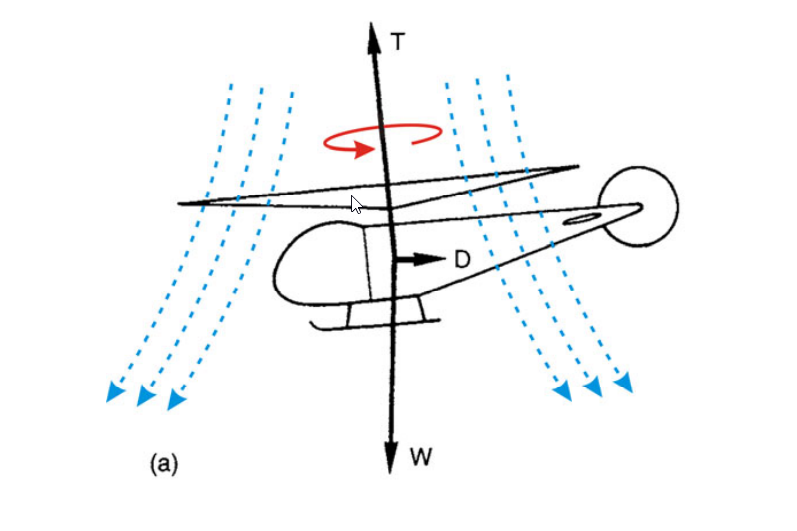
\includegraphics[width= \linewidth]{helicopter.png} & 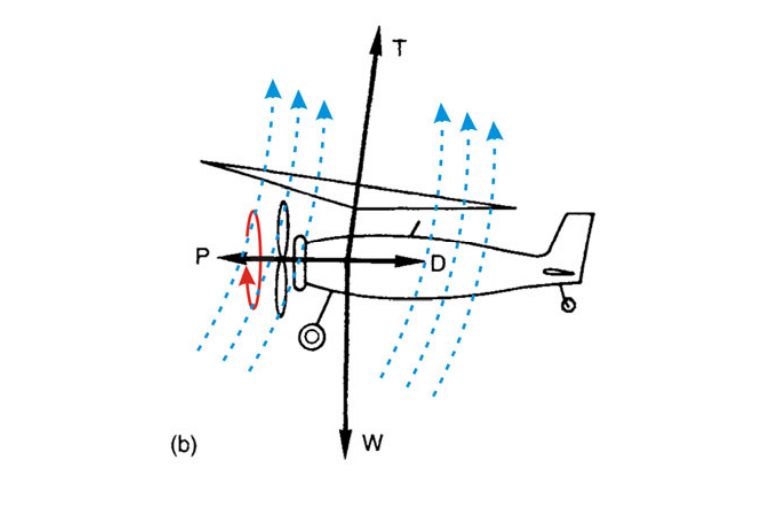
\includegraphics[width=\linewidth]{Autogyro.png}                       &
		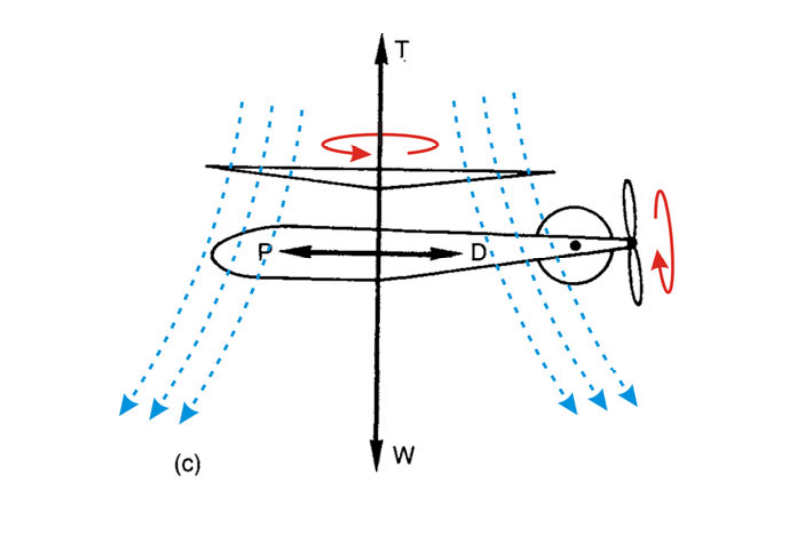
\includegraphics[width= \linewidth]{Gyrodyne.png}                                                                                                                                                                \\
		Has a power driven main rotor, which can be tilted  & Passive main rotor and a forward facing active propeller. Can't hover. & Active main rotor, but can't be tilted. Additional front facing active propeller.
	\end{tabularx}

	\smallskip
	Typical rotorcrafts are: Single Rotors, Multi rotors, Coaxial, Ducted Fan, Omnidirectional Multicopter(movable rotors).

	\subsection{Modelling of Quadrotor}
	\begin{center}
		\textit{Modeling and simulations are important,} \\ \textit{but they must be validated in reality.}

	\end{center}
	\begin{center}
		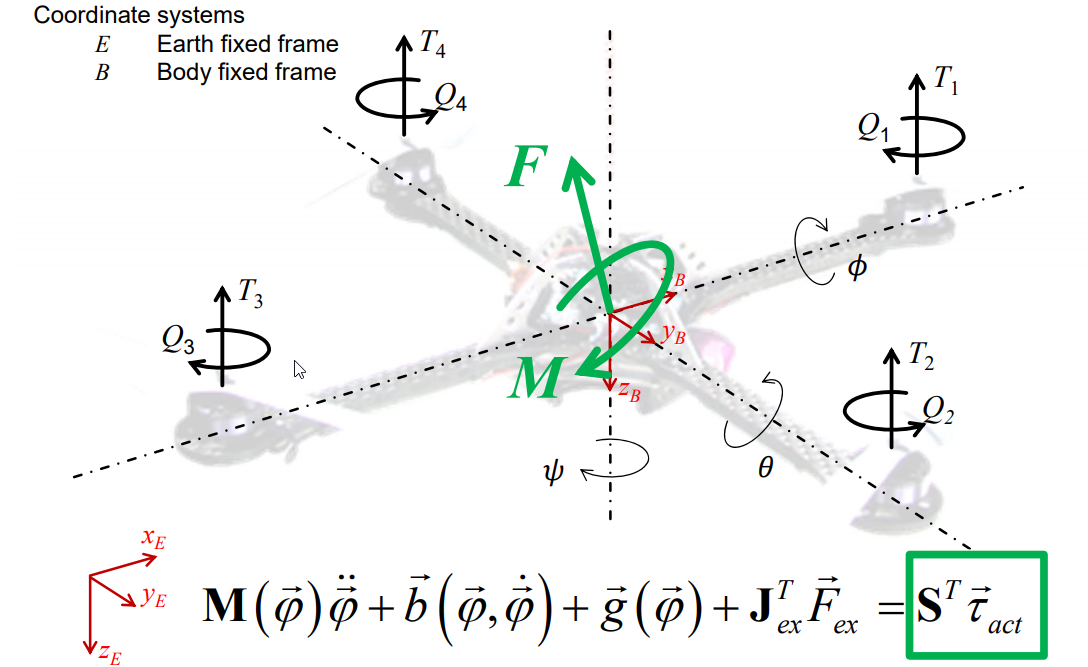
\includegraphics[width=0.8\linewidth]{RotorModelling.png}\\
	\end{center}

	\textbf{Structural Properties:} \\Arm length $l$, Rotor height $h$, Mass $m$, Inertia $I = \left(\begin{smallmatrix}I_{xx} &0 &0\\ 0 & I_{yy} & 0\\ 0 & 0 & I_{zz}\end{smallmatrix}\right)$

	\smallskip
	Hub force \& rolling moments depend on flight regime and can be neglected in hovering.

	\smallskip
	\textbf{Rotation:}\\
	$\begin{pmatrix}\phi \\ \theta \\\psi\end{pmatrix}=\begin{pmatrix}Roll \\ Pitch \\ Yaw\end{pmatrix} \rightarrow \begin{pmatrix}x Axis \\ y Axis \\ z Axis\end{pmatrix} $ with the known rot. matrices.

	\smallskip
	This can be used for a equation for the rotational speed:
	$${}_\mathcal{B}\omega =E_r \dot{\chi_r}=E_r\begin{bmatrix}\dot{\phi}\\\dot{\theta}\\\dot{\psi}\end{bmatrix} \text{, with } E_r = \begin{bmatrix} 1 & 0 & -sin \theta \\ 0 & cos\phi & sin\phi cos\theta \\ 0 & -sin\phi & cos\phi cos \theta\end{bmatrix}$$
	Linearization for small Roll and Pitch ($\phi \approx \theta \approx 0$) results in a \textbf{unity matrix} $E_r = \mathbbm{1}$

	\subsubsection{Body Dynamics}
	$$\begin{bmatrix}
			m\mathbbm{1}_{3\times3} & 0 \\ 0 & I
		\end{bmatrix}
		\begin{bmatrix}
			{}_\mathcal{B}\dot{v} \\ {}_\mathcal{B}\dot{\omega}
		\end{bmatrix}
		+
		\begin{bmatrix}
			{}_\mathcal{B}\omega \times m{}_\mathcal{B}v \\
			{}_\mathcal{B}\omega \times I_\mathcal{B}\omega
		\end{bmatrix}
		=
		\begin{bmatrix}
			{}_\mathcal{B}F \\
			{}_\mathcal{B}M
		\end{bmatrix}
	$$
	with Forces $${}_\mathcal{B}F = {}_\mathcal{B}F_G + {}_\mathcal{B}F_{Aero} = C_{EB}^T
		\begin{bmatrix}
			0 \\ 0\\ mg
		\end{bmatrix}
		+ \sum_{i=1}^4
		\leftidx{_\mathcal{B}}{\begin{pmatrix}
				0 \\0\\ -T_i
			\end{pmatrix}}
	$$\\

	and Hover Moments $${}_\mathcal{B}M_{\text{Aero}} =
		\leftidx{_\mathcal{B}}{\begin{pmatrix}
				l(T_4-T_2) \\ l(T_1-T_3)\\ 0
			\end{pmatrix}}+
		\leftidx{_\mathcal{B}}{\begin{pmatrix}
				0 \\
				0 \\
				\displaystyle\sum_{i=1}^4Q_i(-1)^{(i-1)}
			\end{pmatrix}}
	$$
	with Thrust forces $T_i = b_i\omega_{p,i}^2$ and Drag Forces $Q_i= d_i \omega_{p,i}^2$

	\medskip
	\textbf{Rotational Dynamics} (fist row of Dynamics)
	\begin{align*}
		I_{xx}\dot{\omega}_x & = \omega_y\cdot \omega_z (I_{yy}-I_{zz})+l\cdot b (\omega_{p,4}^2-\omega_{p,2}^2) \\
		I_{yy}\dot{\omega}_y & = \omega_z\cdot \omega_x (I_{zz}-I_{xx})+l\cdot b (\omega_{p,1}^2-\omega_{p,3}^2) \\
		I_{zz}\dot{\omega}_z & = d(\omega_{p,1}^2-\omega_{p,2}^2+\omega_{p,3}^2-\omega_{p,4}^2)                  \\
		                     & \text{with $\omega_{xyz}$ as entries of the body rotation ${}_\mathcal{B}\omega$}
	\end{align*}
	$\Rightarrow$ We have full control over all rotational speeds (every equation depends on rotor speeds $w_{p,i}$). Note that $(I_{xx}-I_{yy})=0$ (x-y symmetry), which dropped out of the 3rd equation.

	\medskip
	\textbf{Translational Dynamics} (2nd row of dynamics)
	\begin{align*}
		m\dot{v}_x = & m(\omega_z\cdot v_y - \omega_y\cdot v_z)\textcolor{blue}{-sin\theta mg}                                     \\
		m\dot{v}_y = & m(\omega_x\cdot v_z - \omega_z\cdot v_x)\textcolor{blue}{+sin\phi cos\theta mg}                             \\
		m\dot{v}_z = & m(\omega_y\cdot v_x - \omega_x\cdot v_y) \textcolor{blue}{+cos\phi cos\theta mg }                           \\
		             & - b(\omega_{p,1}^2+\omega_{p,2}^2+\omega_{p,3}^2+\omega_{p,4}^2)                                            \\
		             & \text{with gravitational Terms in \textcolor{blue}{blue}, } {}_\mathcal{B}F_G=C_{EB}^T\cdot {}_E\vec{n}_zmg
	\end{align*}
	$\Rightarrow$ Only z-Axis can be controlled directly with $\omega_{p,i}$

	\smallskip
	\textcolor{red}{Note: To be consistent with the lecture notation: $(\omega_x, \omega_y, \omega_z) = (p,q,r) $ and $(v_x, v_y, v_z) = (u, v, w)$}

	\subsection{Control of a Quadrotor}

	The system has 6 DoF, but only 4 Inputs (Motors) $\rightarrow$ \textbf{Under-actuated}! \\
	$\Rightarrow$ Forward Motion requires tipping around Roll and Pitch.

	\textbf{Define Virtual control inputs:}\\
	By defining a new set of inputs, we can decouple the Dynamic equations

	\begin{minipage}{0.4\linewidth}
		\begin{center}
			Total Thrust
		\end{center}
		\begin{align*}
			U_1 = & b(\omega_{p1}^2+\omega_{p2}^2 \\
			      & +\omega_{p3}^2+\omega_{p4}^2)
		\end{align*}

	\end{minipage}\hfill
	\begin{minipage}{0.55\linewidth}
		\begin{center}
			Moments along axis
		\end{center}
		$U_2 = l\cdot b(\omega_{p4}^2-\omega_{p2}^2)$\\
		$U_3 = l\cdot b(\omega_{p1}^2-\omega_{p3}^2)$\\
		$U_4 = d(\omega_{p1}^2-\omega_{p2}^2+\omega_{p3}^2-\omega_{p4}^2)$
	\end{minipage}

	\smallskip
	which simplify the dynamics from above.

	\smallskip
	\textbf{Linearize Attitude Dynamics}\\
	Linearization around the Equilibrium ($\omega_{x,y,z} = \phi = \theta = U_{2,3,4} = 0; U_1 = mg$) gives further simplification (Recall: $E_r=\mathbbm{1} \Rightarrow \ddot{\chi_r} = [\ddot{\phi} \; \ddot{\theta} \;\ddot{\psi}]^T$): $\Rightarrow$ Can use 3 individual controller
	\boxed{$$
			\dot{\omega}_x = \ddot{\phi} = \frac{1}{I_{xx}}U_2
			\quad
			\dot{\omega}_y = \ddot{\theta} = \frac{1}{I_{yy}}U_3
			\quad
			\dot{\omega}_z = \ddot{\psi} = \frac{1}{I_{zz}}U_4
		$$}


	\smallskip
	\textbf{Altitude Control:}\\
	%%somethings feels wrong in here (and the slides)
	Dynamics from above, but in \textit{Inertial Frame}:
	$$\dot{v}_z = \ddot{z} = g- cos\phi cos\theta \frac{1}{m}U_1 =: g- \frac{1}{m}T_z $$
	Now we can derive the input $U_1$ for a chosen controller $T_z$ (representing the Thrust in the inertial frame) :
	$$T_z = -k_p(z_{des}-z)+k_d\dot{z} -mg \Rightarrow U_1 = \frac{T_z}{cos\phi cos\theta}$$

	\smallskip
	\textbf{Position Control:}\\
	We can use 3 separate PD Controller to get the trust for x,y and z in the inertial frame.
	$$\text{Dynamics } \Rightarrow \setlength\arraycolsep{2pt}\begin{bmatrix}\ddot{x} &\ddot{y}&\ddot{z} \end{bmatrix}^T = \frac{1}{m}\begin{bmatrix}T_x&T_y&T_z \end{bmatrix}^T + \begin{bmatrix}0 &0 &g \end{bmatrix}^T$$
	This must be transformed to get the desired Total thrust as well as roll and pitch angles.
	$$T = \sqrt{T_x^2+T_y^2+T_z^2} \quad \& \quad \frac{1}{T} C_{E1}^T(z,\psi)
		\begin{bmatrix}
			T_x \\ T_y \\ T_z
		\end{bmatrix}
		=
		\begin{bmatrix}
			sin\theta cos\phi \\ -sin\phi \\ cos\theta cos\phi
		\end{bmatrix}$$
	\textbf{Remark:} $C_{E1}(z,\psi)$ is the rotation matrix around $z$ with angle $\psi$.\\
	\textbf{Remark2:} $\left[\begin{smallmatrix} sin\theta cos\phi  \\ -sin\phi \\ cos\theta cos\phi \end{smallmatrix}\right]$ describes the Thrust of the Quadrotor in the Inertial frame (can only apply thrust perpendicular to the rotors). \\
	It's calculated with $C_{12}(y,\theta)\cdot C_{2B}(x,\phi)\cdot (0,0,1)^T$
	\subsection{Propeller Aerodynamics}
	There are 4 main forces generated by the rotor:

	\medskip
	\textbf{For a Rotor in Hover:}

	\smallskip
	\begin{minipage}{0.45\linewidth}
		Thrust Force T

		\smallskip
		Aerodynamic force perpendicular to rotor plane

		\smallskip
		$|T|=\frac{\rho}{2}A_PC_T(\omega_pR_P)^2$

	\end{minipage}\hfill
	\begin{minipage}{0.5\linewidth}
		Drag Torque Q

		\smallskip
		Torque around rotor plane

		\smallskip
		$|Q|=\frac{\rho}{2}A_PC_Q(\omega_pR_P)^2R_P$

	\end{minipage}

	\medskip
	\textbf{For a Rotor in forward flight:}

	\begin{minipage}{0.45\linewidth}
		Hub force H

		\smallskip
		Opposite to horizontal flight direction $V_H$

		\smallskip
		$|H|= \frac{\rho}{2}A_PC_H(\omega_pR_P)^2$
	\end{minipage}\hfill
	\begin{minipage}{0.5\linewidth}
		Rolling Moment R

		\smallskip
		Around flight direction

		\smallskip
		$|R|= \frac{\rho}{2}A_PC_R(\omega_pR_P)^2R_P$
	\end{minipage}


	\subsubsection{Momentum Theory}
	{\small
		$\rho:\text{fluid density, }\vec{V}:\text{flow speed, } \vec{n}: \text{surface normal, }$

		$dA: \text{surface Area patch, } p: \text{ surface pressure, } E: \text{ Energy, } P: \text{ Power}$
	}

	\smallskip
	\begin{minipage}{0.6\linewidth}
		Conservation of fluid mass
		$$\displaystyle \iint \rho\vec{V}\cdot \vec{n}dA = 0 $$

		Conservation of fluid Momentum:
		$$\displaystyle \iint p\cdot \vec{n}dA+\iint (\rho\vec{V})\vec{V}\cdot \vec{n}dA = \vec{F} $$

		Conservation of energy:
		$$\displaystyle \iint\frac{1}{2}\rho V^2\vec{V}\cdot \vec{n}dA=\frac{dE}{dt}=P$$

	\end{minipage}\hfill
	\begin{minipage}{0.38\linewidth}
		Mass flow inside and outside (closed) control Volume must be equal

		\bigskip
		The net Force is the change of momentum of the fluid

		\bigskip
		Work done on the fluid results in a gain of kinetic energy

	\end{minipage}

	\smallskip
	\begin{minipage}{0.35\linewidth}
		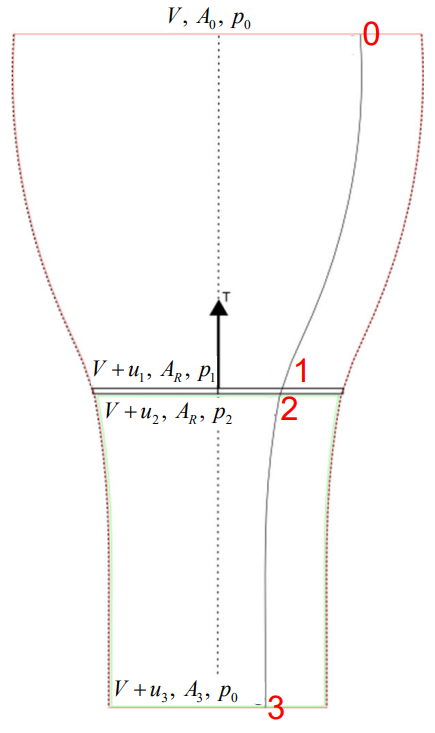
\includegraphics[width=\linewidth]{1danalysis.png}
	\end{minipage}\hfill
	\begin{minipage}{0.6\linewidth}
		\textbf{1D Analysis:}

		\medskip
		The formulas lead to the following results:

		$\rho A_0 V = \rho A_R (V+u_1)$

		$\quad = \rho A_R (V+u_2)= \rho A_R (V+u_3)$

		$\Rightarrow u_1=u_2$

		\smallskip
		$F_{\textit{Thrust}} = \rho A_R(V+u_1)u_3$

		$P_{\textit{Thrust}} = F_{\textit{Thrust}}(V+u_1) $

		$\quad= \frac{1}{2}\rho A_R(V+u_1)(2V+u_3)u_3$

		$\Rightarrow = u_3 = 2u_1$

		\smallskip
		\textbf{In the Hover case ($V=0$):}

		Thrust Force: $F_{\textit{Thrust}} = 2\rho A_Ru_1^2$

		Slipstream Tube: $A_0 = \infty \quad A_3 = \frac{A_R}{2}$
	\end{minipage}

	Combining $P=F_{\textit{Thrust}}(\overbrace{V}^{=0}+u_1)$ with $F_{\textit{Thrust}}=2\rho A_Ru_1^2$ gives the ideal Power to Hover:
	$$P=\frac{F_{\textit{Thrust}}^{3/2}}{\sqrt{2\rho A_R}} = \frac{(mg)^{3/2}}{\sqrt{2\rho A_R}} \text{ with } F_{\textit{Thrust}} = mg$$
	The Power depends on the \textbf{Disc Loading} $F_{\textit{Thrust}}/A_R$

	\smallskip
	\textbf{Defining the rotor efficiency, Figure of Merit}, $FM$\\
	$$FM = \frac{\textit{Ideal power to hover}}{\textit{Actual power to hover}}<1$$
	$\rightarrow$ compare different propellers with the same disc loading.

	%%%%%%%%%%%%%%%%%%%%%%%%%%%%%%%%%%%%%%%%%%%%%%%%%%%%%%%%%%%%%%%%%%%%%%%%%%%%%%%%%%%%%%%%%%%%%%%%%%%%%%
	%   _____           _   _               _____ 
	%  / ____|         | | (_)             | ____|
	% | (___   ___  ___| |_ _  ___  _ __   | |__  
	%  \___ \ / _ \/ __| __| |/ _ \| '_ \  |___ \ 
	%  ____) |  __/ (__| |_| | (_) | | | |  ___) |
	% |_____/ \___|\___|\__|_|\___/|_| |_| |____/ 
	%                                             
	%%%%%%%%%%%%%%%%%%%%%%%%%%%%%%%%%%%%%%%%%%%%%%%%%%%%%%%%%%%%%%%%%%%%%%%%%%%%%%%%%%%%%%%%%%%%%%%%%%%%%%%%%%%%%%%%%%%%
	\section{Case Study: Micro Aerial Vehicles}
	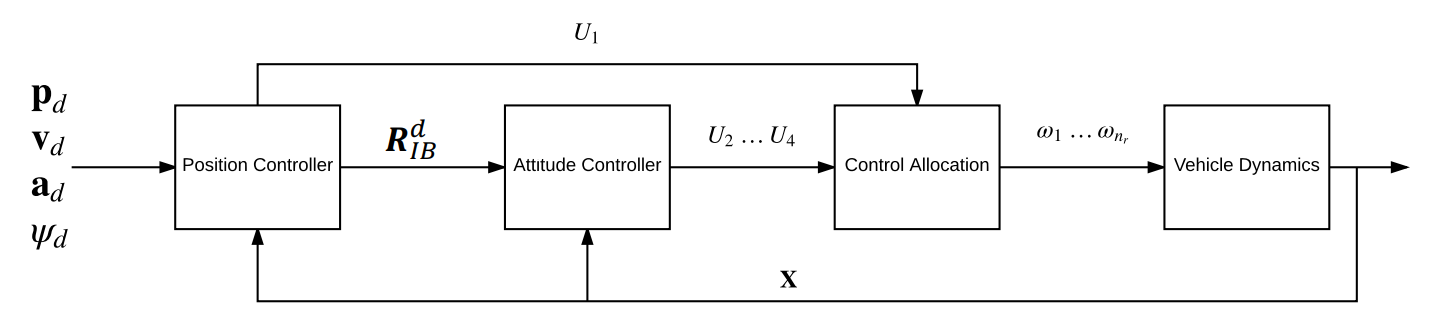
\includegraphics[width = \linewidth]{CaseControlArch.png}
	\subsection{Control for MAVs}

	\textbf{Virtual Control Input (allocation):}\\
	$$\left(\begin{smallmatrix}
				U_1 \\U_2\\U_3\\U_4
			\end{smallmatrix}\right) = A \begin{pmatrix}
			\omega^2_1 \\ ...\\\omega^2_{n_r}
		\end{pmatrix} , \quad A\in \mathbb{R}^{4\times n_r}$$



	\subsubsection{Trajectory Tracking Controller}
	Error definitions: Position $e_p = p-p_d$, Velocity $e_v = v - v_d$
	$$z_B^d = \frac{-K_pe_p-K_ve_v-m(g-a_d)}{||-K_pe_p-K_ve_v-m(g-a_d)||}$$
	$${}_Ix_{temp}^d =
		\begin{pmatrix}
			cos\psi_d \\sin\psi_d\\0
		\end{pmatrix}
		\quad {}_Iy_B^d = \frac{{}_Iz_B^d\times {}_Ix^d_{temp}}{||{}_Iz_B^d\times {}_Ix^d_{temp}||}$$
	From this we can construct the Rotation Matrix  $\mathbf{R_{IB}^d= [{}_Iy_B^d\times {}_Iz_B^d ,\; {}_Iy_B^d ,\;  {}_Iz_B^d]}$

	\textbf{Note:} ${}_Ix_{temp}^d$ is generally not perpendicular to ${}_Iz_B^d$, so we use some orthogonal projections for the first entry of $\mathbf{R_{IB}^d}$

	\smallskip
	\textbf{Attitude Control}
	$$\begin{pmatrix}
			U_2 \\U_3\\U_4
		\end{pmatrix} = -K_Re_R -K_\omega e_\omega + \omega\times J\omega$$
	with errors: $$\mathbf{e_R} = \frac{1}{2}\left((R_{IB}^d)^TR_{IB}-R_{IB}^TR_{IB}^d\right)^\vee,
		\mathbf{e_\omega} = \omega -R_{IB}^TR_{IB}^d\omega_d$$
	where $(.)^\vee$ maps the cross product matrix to a vector.

	\smallskip
	\textbf{Trajectory Tracking}

	Project Thrust onto Body z-Axis:
	$$U_1 = (-K_pe_p-K_ve_v-m(g-a_d) )\cdot{}_I\vec{n}_{z,B}$$

	%%%%%%%%%%%%%%%%%%%%%%%%%%%%%%%%%%%%%%%%%%%%%%%%%%%%%%%%%%%%%%%%%%%%%%%%%%%%%%%%%%%%%%%%%%%%%%%%%%%%%%
	%   _____           _   _                 __  
	%  / ____|         | | (_)               / /  
	% | (___   ___  ___| |_ _  ___  _ __    / /_  
	%  \___ \ / _ \/ __| __| |/ _ \| '_ \  | '_ \ 
	%  ____) |  __/ (__| |_| | (_) | | | | | (_) |
	% |_____/ \___|\___|\__|_|\___/|_| |_|  \___/ 
	%%%%%%%%%%%%%%%%%%%%%%%%%%%%%%%%%%%%%%%%%%%%%%%%%%%%%%%%%%%%%%%%%%%%%%%%%%%%%%%%%%%%%%%%%%%%%%%%%%%%%%%%%%%%%%%%%%%%
	\section{Fixed Wing UAVs}
	\subsection{Basic Principles}
	For incompressable and non viscous fluids, we can use the Bernoulli Equation:
	$\frac{v^2}{2}+gh+\frac{p}{\rho} = const.$
	This results in a \textcolor{green}{Lift} and a \textcolor{magenta}{Drag} Force with an additional \textcolor{blue}{Moment} on the Airfoil. Lift/Drag is always perpendicular/parallel to the air velocity!\\
	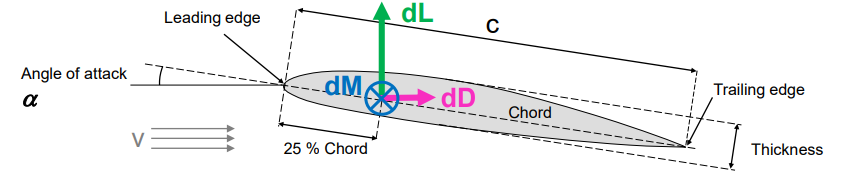
\includegraphics[width=\linewidth]{Aerodynamics.png}
	\begin{description}
		\item[Stall Point:] The angle of attack at which the maximum lift occurs. (Flow will separate for higher $\alpha$)
	\end{description}

	\subsection{Fixed Wing Kinematics}
	\begin{description}
		\item[Assumptions:] Aerodynamics where we don't enter Stall, neglect side-forces and interference effects
		\item[Inertial frame:] X-Axis: North;
		      Y-Axis: East;
		      Z-Axis: Downwards

		\item[Body-fixed frame:]X-Axis: out of the nose;
		      Y-Axis: out of the \textbf{right} wing;
		      Z-Axis: Downwards; The Orientation of the Body Frame is describes as usual in Euler Angles with roll, pitch and yaw $\rightarrow \phi, \theta,\psi$.
	\end{description}

	\textbf{Control Surfaces:} The standard Control surfaces are \textbf{Elevator} (pitch), \textbf{Aileron} (roll), \textbf{Rudder} (yaw).

	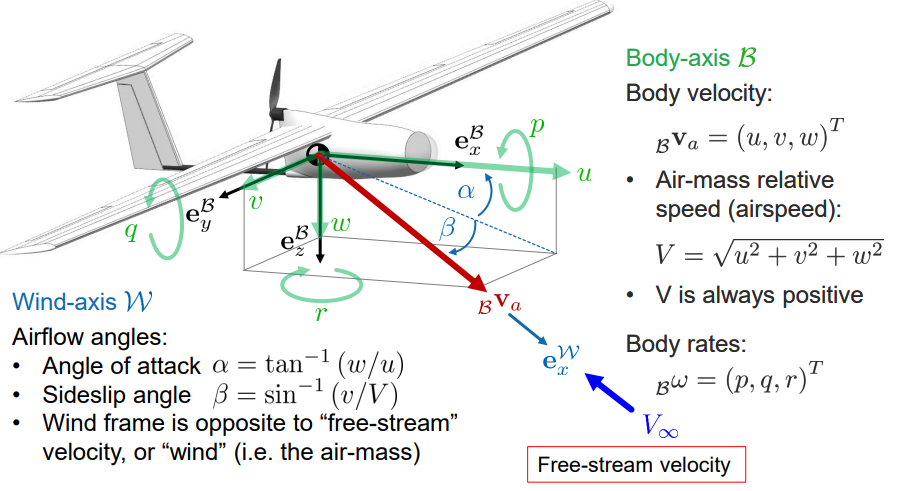
\includegraphics[width=0.8\linewidth]{Fixedwing_kin.png}\\

	\textbf{Flight Path Angle:} $\gamma$, defined from horizon to ${}_\mathcal{I}v_a$

	\textbf{Heading Angle:} $\xi$, defined from North to ${}_\mathcal{I}v_a$

	\textbf{Course Angle:} $\chi$, defined from North to ${}_\mathcal{I}v = {}_\mathcal{I}v_a + {}_\mathcal{I}v_{wind}$

	\subsection{Fixed Wing Dynamics}
	\subsubsection{Forces}

	\textbf{Non Aerodynamics:} Weight, Propeller Thrust.

	\textbf{Aerodynamic:} $$\text{Lift: }L=\frac{1}{2}\rho V^2Sc_L, \quad \text{Drag: } D=\frac{1}{2}\rho V^2Sc_D $$ with surface $S$.

	Note: $c_L$ and $c_D$ are dependent on $\alpha$, Side-Forces: assumed zero

	\subsubsection{Equations of Motion, ($I_{xz}$ is typically small)}
	$${}_\mathcal{B}\dot{v}_a= \frac{1}{m}\sum{}_\mathcal{B}F - {}_\mathcal{B}\omega \times {}_\mathcal{B}v_a, \quad {}_\mathcal{I}\dot{r}=C_\mathcal{IB} {}_\mathcal{B}v_a+{}_\mathcal{I}v_w$$
	$${}_\mathcal{B}\dot{\omega}={}_\mathcal{B}I^{-1}\left(\sum {}_\mathcal{B}M -{}_\mathcal{B}\omega \times ({}_\mathcal{B}I{}_\mathcal{B}\omega)\right), \; {}_\mathcal{B}I = \left[\begin{smallmatrix}I_{xx} & 0 & I_{xz}\\ 0 & I_{yy} & 0 \\ I_{xz} & 0 & I_{zz}\end{smallmatrix}\right]$$

	\subsection{Cascaded Control Loops}
	\subsubsection{Steady Level Turning}
	We need ${}_\mathcal{B}\dot{v}_a = {}_\mathcal{B}\dot{\omega}=0$ ;  $\theta = \alpha \rightarrow \gamma = 0$ and $\phi = const \neq 0$.

	\begin{itemize}
		\item[-] The Lift $L$ increases with $\frac{1}{cos\phi}$ \quad $\leftarrow$ ($ L = \frac{mg}{cos\phi} $)

		\item[-] The air speed $V_{min}$ increases with $\sqrt{1/cos\phi}$ \quad $\leftarrow$ $(\frac{1}{2}\rho V^2Sc_L = L$)
	\end{itemize}
	The Heading rate $\xi$ can be found with a force balance with the centripetal force (and $\dot{\psi}\approx \dot{\xi}$). Note: $\dot{\xi} = V/R \Leftrightarrow v=r\cdot \omega $
	$$F_{cent}= m\frac{V_{G}^2}{R}= L\cdot sin\phi \; \&\; L\cdot cos\phi = mg \Rightarrow \dot{\psi}= \dot{\xi} = \frac{g}{V}tan\phi$$

	\textbf{Lateral-directional path}\\
	\begin{minipage}{0.4\linewidth}
		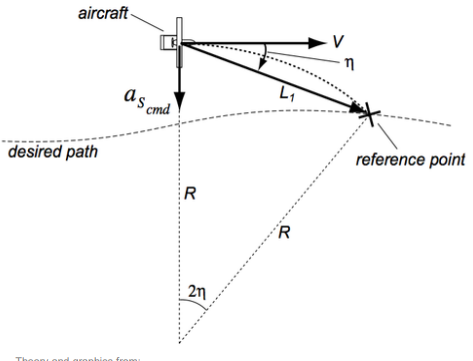
\includegraphics[width=\linewidth]{lateral.png}
	\end{minipage}
	\begin{minipage}{0.6\linewidth}
		$sin\eta = \frac{L_1}{2R} \Rightarrow R= \frac{L_1}{2sin\eta}$

		$a_{s_{cmd}}= \frac{V^2}{R}= 2\frac{V^2sin\eta}{L_1} \Rightarrow \dot{\xi}_d=\frac{a_{s_{cmd}}}{V}$

		\smallskip
		with the above:

		$\displaystyle \phi = tan^{-1}\left(\frac{a_{s_{cmd}}}{g}\right)$

		So we can get the needed roll angle for a desired turn with velocity $V$.
	\end{minipage}


	\subsubsection{TECS - Total Energy Control System}

	$$\dot{E}_{spec}= \frac{\dot{V}}{g}+sin\gamma \approx \frac{\dot{V}}{g}+\gamma, \quad \dot{E}_{dist} = \gamma - \frac{\dot{V}}{g}
	$$
	'\textit{Potential energy rate minus kinetic energy rate}'



	%%%%%%%%%%%%%%%%%%%%%%%%%%%%%%%%%%%%%%%%%%%%%%%%%%%%%%%%%%%%%%%%%%%%%%%%%%%%%%%%%%%%%%%%%%%%%%%%%%%%%%
	%	                                    _ _      
	%     /\                               | |(_)     
	%    /  \   _ __  _ __   ___ _ __   __| |___  __
	%   / /\ \ | '_ \| '_ \ / _ \ '_ \ / _` | \ \/ /
	%  / ____ \| |_) | |_) |  __/ | | | (_| | |>  < 
	% /_/    \_\ .__/| .__/ \___|_| |_|\__,_|_/_/\_\
	%          | |   | |                            
	%          |_|   |_| 
	%%%%%%%%%%%%%%%%%%%%%%%%%%%%%%%%%%%%%%%%%%%%%%%%%%%%%%%%%%%%%%%%%%%%%%%%%%%%%%%%%%%%%%%%%%%%%%%%%%%%%%%%%%%%%%%%%%%%



\end{multicols*}
\end{document}
